\documentclass[11pt, letterpaper]{article}
\usepackage[margin=0.5in]{geometry}
\usepackage{graphicx}

\begin{document}

\title{String Search}
\author{Ryan Layer}
\maketitle

\section{Introduction}
An organism's DNA encompasses all instructions for its development and
function. To link specific DNA sequences to particular traits or diseases, we
analyze the DNA of individuals exhibiting similar or differing characteristics.
DNA's structure—a long sequence of nucleotides denoted by A, C, T, and
G—transforms the comparison of two genomes into a computational string search
challenge. This problem involves two input strings: a typically longer string,
the text $T$, and a usually shorter string, the pattern $P$. The
objective is to locate every instance of $P$ within $T$. Here we analyze the
the efficiency and memory consumption of a basic string search algorithm that
aligns $P$ with all possible positions in $T$.  The algorithm's runtime
correlated with $T$'s length and it's additional memory requirement were
minimal.

\section{Results}

As expected, the runtime of the naive string search algorithm increased
linearly and the memory usage remained constant as the text size increased
(Figure~\ref{timeandmem}). The algorithm's runtime increased linearly with
the text size because the algorithm considers all possible alignments of the
pattern $P$ with the text $T$. As the text size increases, the number of
possible alignments increases linearly. The algorithm's memory usage remained
constant because the algorithm only stores the positions of the pattern $P$ in
the text $T$.

%%%%% Add your experiment here %%%%

\begin{figure}[ht] \centering
    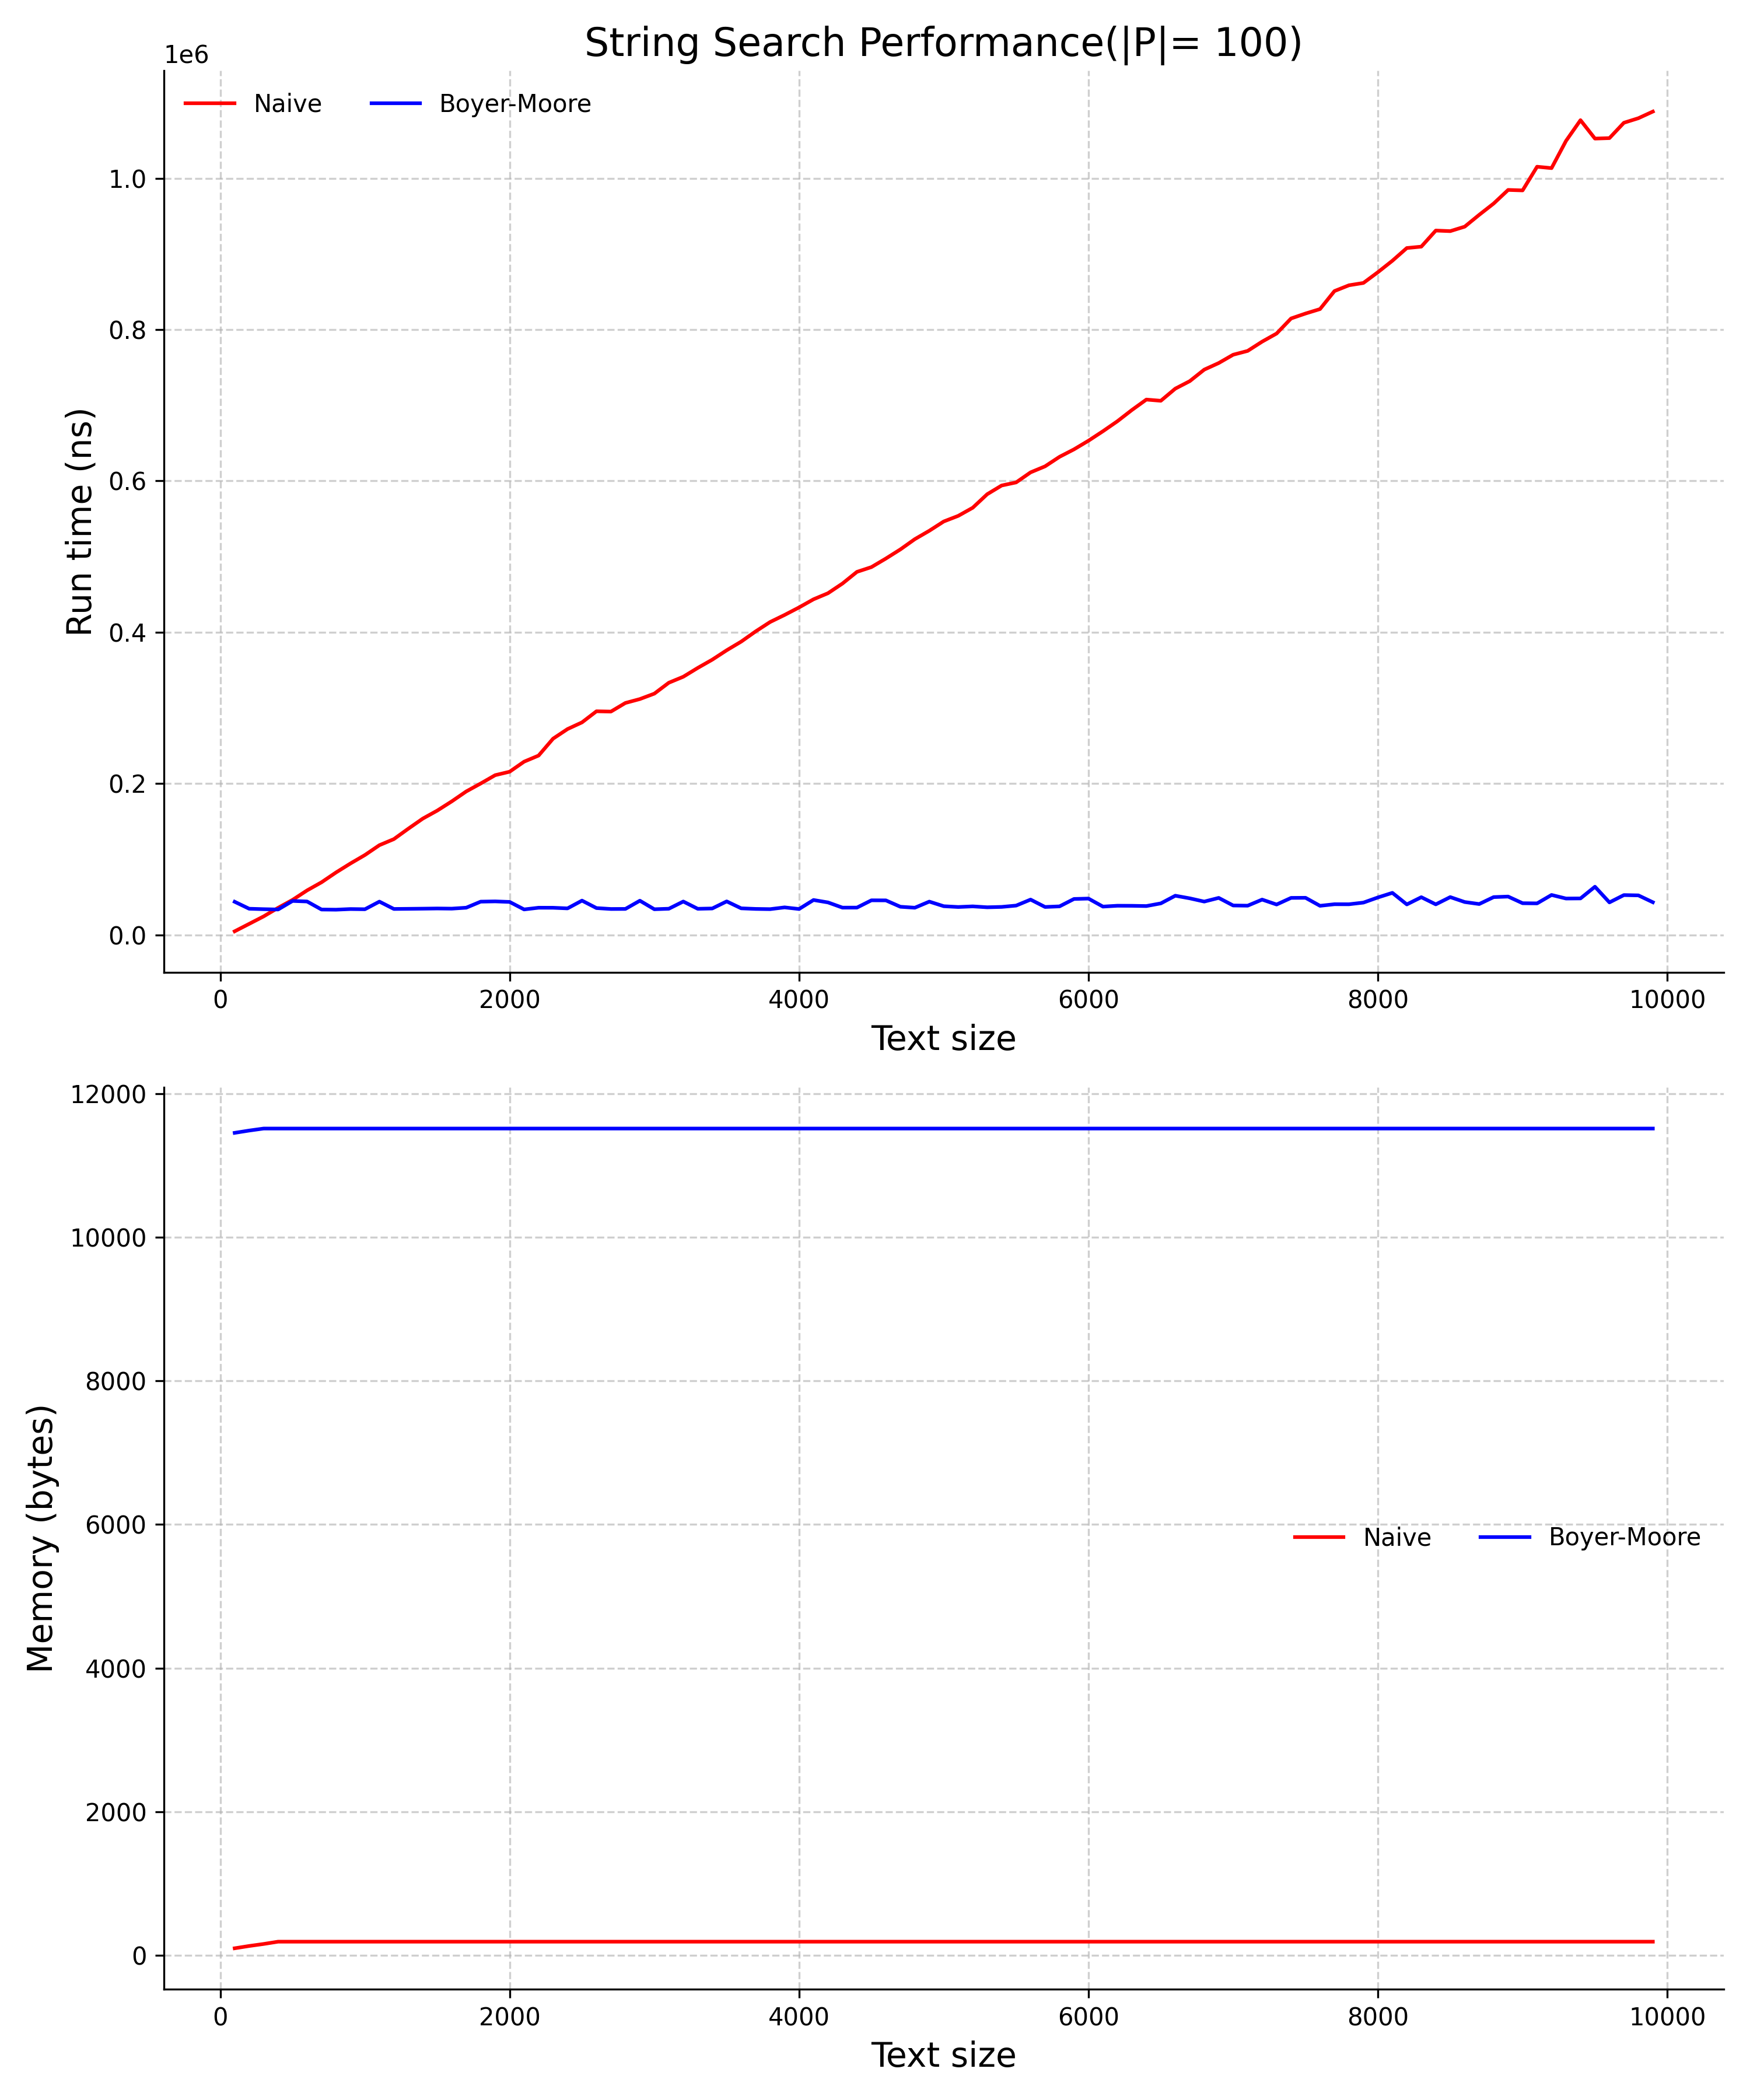
\includegraphics[width=0.6\textwidth]{naive_search}
    \caption{The empirical runtime and memory usage of the naive string search
    algorithm considering a pattern size of 100 and a database size ranging
    from 100 to 10,000 characters.}
    \label{timeandmem}
\end{figure}

%%%% Add your figure here %%%%

\section{Methods}

\subsection{Naive string search}
The naive string search algorithm considers all possible alignments of the
pattern $P$ with the text $T$. Staring at the first position in $T$, the
algorithm compares $P$'s characters with the corresponding characters in $T$.
If all characters match, the algorithm records the alignment's position in $T$.
The algorithm then repeats this process for the next alignment. If any of the 
characters in $P$ do not match a corresponding character in $T$, the current
alignment breaks and then $P$ shifts down one position in $T$, and the process
repeats. This process continues until $P$ has been compared to all possible
alignments in $T$, then returns the recorded positions.

\subsection{Empirical comparison}

We evaluated the performance of the naive string search algorithm considering a
pattern size of 100 and text sizes that ranged from 100 to 10,000 characters
with a step size of 100.  The performance metrics include runtime and memory
usage. For each text size, we ran a single search where we generated a random
string for $T$ from the alphabet ${A, C, T, G}$ and extracted a random
substring $P$ from $T$. We then recorded the runtime and memory usage of the
algorithm consiuder that $P$ and $T$. After the round was complete for a given
text size, we calculated the average runtime and memory usage for the search.

\subsection{Reproducibility}
To replicate these experiments, clone the repository and then run the
following commands from the root directory of the repository.
\begin{verbatim}
$ git clone https://github.com/ryanlayerlab/string_search.git
$ cd string_search
$ python src/string_search.py \
    --text_range 100 10000 100 \
    --pattern_size 100 \
    --rounds 1 \
    --out_file doc/naive_search.png
\end{verbatim}
%%%% Add your command here%%%%

\end{document}
